\section{Evaluation}

\begin{comment}

  \begin{table*}
    %  \renewcommand{\arraystretch}{1.3}
    \centering
    \caption{Results of aspect transformations on the original MaxC
      design for the RTM kernel.}
    \label{table:feature-comparison}
    \begin{tabular}{ p{2cm}  | p{1cm} | c|  p{1cm} |  p{1cm} |  p{1cm} |  p{1cm} | c | p{1cm} |c | c | c}
      Aspect                           & DSP Balance    & Par & LUT               & FF                & BRAM           & DSP            & Frequency & Compile Time & LOC & Speedup & Throughput \\ \hline
      \multirow{4}{*}{OptimizeDSPUsage} & none           & 1   & 67327 (22.62\%)   & 92607  (15.56\%)  & 248 (23.31\%)  & 0  (0.00\%)    & 303/100   & 2 h 9        & LOC & Speedup & Throughput \\
      & balanced       & 1   & 59202 (19.89\%)   & 84101 (14.13\%)   & 248 (23.31\%)  & 34 / (1.69\%)  & 303/100   & 1h 49        & LOC & Speedup & Throughput \\
      & full           & 1   & 52619  (17.68\%)  & 76107  (12.79\%)  & 248  (23.31\%) & 117  (5.80\%)  & 303/100   & 2 h 2        & LOC & Speedup & Throughput \\ \hline
      & none           & 2   & 92109 (30.95\%)   & 122224 (20.53\%)  & 261 (24.53\%)  & 0 (0.00\%)     & 303/100   & 3h5          & LOC & Speedup & Throughput \\
      & balanced       & 2   & 75719 (25.44\%)   & 75719 (25.44\%)   & 261 (24.53\%)  & 68 (3.37\%)    & 303/100   & 2h30         & LOC & Speedup & Throughput \\
      & full           & 2   & 63032  (21.18\%)  & 89284  (15.00\%)  & 260  (24.44\%) & 234  (11.61\%) & 303/100   & 2 h 8        & LOC & Speedup & Throughput \\
      \hline
      & none           & 3   & 116532 (39.16\%)  & 152406 (25.61\%)  & 256 (24.06\%)  & 0 (0.00\%)     & 303/100   & 3 h 20       & LOC & Speedup & Throughput \\
      & balanced       & 3   & 93911 (31.56\%)   & 126888 (21.32\%)  & 256 (24.06\%)  & 102 (5.06\%)   & 303/100   & 2h30         & LOC & Speedup & Throughput \\
      & full           & 3   & 74575  (25.06\%)  & 102965  (17.30\%) & 255  (23.97\%) & 351  (17.41)\% & 303/100   & 2 h 18       & LOC & Speedup & Throughput \\
      \hline
      & \TODO none     & 6   & 116532 (39.16\%)  & 152406 (25.61\%)  & 256 (24.06\%)  & 0 (0.00\%)     & 303/100   & 3 h 20       & LOC & Speedup & Throughput \\
      & \TODO balanced & 6   & 92109 (30.95\%)   & 122224 (20.53\%)  & 261 (24.53\%)  & 0 (0.00\%)     & 303/100   & 3h5          & LOC & Speedup & Throughput \\
      & full           & 6   & 106033  (35.63\%) & 143508  (24.11\%) & 295  (27.73\%) & 702  (34.82\%) & 303/100   & 3h 42        & LOC & Speedup & Throughput \\
    \end{tabular}
  \end{table*}

  \begin{table*}
    % \renewcommand{\arraystretch}{1.3}
    \centering
    \caption{Results of aspect transformations on the original MaxC
      design for the RTM kernel.}
    \label{table:feature-comparison}
    \begin{tabular}{ p{2cm}  | p{1cm} | c|  p{1cm} |  p{1cm} | p{1cm} |   p{1cm} |  p{1cm} | c | p{1cm} |c | c | c}
      Aspect                               & Word Width & Burst & Par & LUT               & FF                & BRAM                 & DSP             & Frequency & Compile Time & LOC & Speedup & Throughput \\ \hline
      \multirow{4}{*}{Optimize word width} & 8, 24      & 64    & 2   & 63447  (21.32\%)  & 89150  (14.98\%)  & 260  (24.44\%))      & 234  (11.61\%)  & 400/100   & 2 h 30       & LOC & Speedup & Throughput \\
      & 8, 24      & 64    & 3   & 75676  (25.4\%)   & 102831  (17.28\%) & 255  (23.97\%)       & 351  (17.41\%)  & 400/100   & 2 h 35       & LOC & Speedup & Throughput \\
      & 8, 24      & 64    & 6   & 101578  (34.13\%) & 143374  (24.09\%) & 248          295  (27.73\%) & 702  (34.82\%)  & 400/100   & 4 h 17       & LOC & Speedup & Throughput \\ \hline
      & 8, 24      & 1     & 6   & 106033  (35.63\%) & 143508  (24.11\%) & 295  (27.73\%)       & 702  (34.82\%)  & 303/100   & 3h 42        & LOC & Speedup & Throughput \\
      & 8, 22      & 1     & 6   & 133973  (45.02\%) & 185520  (31.17\%) & 295  (27.73\%)       & 306  (15.18\%)  & 303/100   & 3 h 13       & LOC & Speedup & Throughput \\
      & 8, 20      & 1     & 6   & 129581  (43.54\%) & 178333  (29.96\%) & 289  (27.16\%)       & 306  (15.18\%)  & 303/100   & 3 h 30       & LOC & Speedup & Throughput \\ \hline
      & 8, 18      & 1     & 6   & 121439  (40.81\%) & 170721  (28.68\%) & 286  (26.88\%)       & 306  (15.18\%)) & 303/100   & 3h 19        & LOC & Speedup & Throughput \\
      & 8, 16      & 1   & 6   & 117904  (39.62\%) & 157359  (26.44\%) & 283  (26.60\%)       & 204  (10.12\%)  & 400/100   & 2 h 50       & LOC & Speedup & Throughput \\ \hline

    \end{tabular}
  \end{table*}
\end{comment}


\subsection{RTM}
We evaluate the proposed approach by implementing a high-performance
application based on the Reverse Time Migration method for seismic
imaging which is used to detect geological structures, based on the
Earth's response to injected acoustic waves. The technique models the
propagation of injected waves using the isotropic acoustic wave
equation \cite{araya2011assessing}:
\begin{align}
\frac{d^2p(r,t)}{dt^2} + {dvv(r)}^2\bigtriangledown^2p(r,t) = f(r,t)
\end{align}
We approximate the differential equation using stencil computation to
perform a fifth-order Taylor expansion in space and first-order Taylor
expansion in time. We use MaxC to implement the dataflow kernel and
aspects to generate multiple configurations for the design.

\subsection{Results}


Results of the design space exploration using the word length aspect
illustrate the trade-offs between accuracy and resource usage as shown
in Figure \ref{fig:precision}.  We observe irregular, large variations
when decreasing the mantissa from 18 16 and 24 to 22. The latter
difference is unexpected, halving the number of required DSPs
(although increasing the LUT and FF usage by 30\%), with little impact
on accuracy. This is the effect of the backend tools implementing
arithmetic operations using a combination of both DSPs and LUT/FF
elements. The mantissa boundaries at which this optimization occurs
are platform specific (depending on the architecture of the
DSPs). Hence automating this optimization via aspects and decoupling
it from the original source code makes the application more portable
and facilitates discovery of interesting trade-off opportunities using
design space exploration.

\begin{figure}[!h]
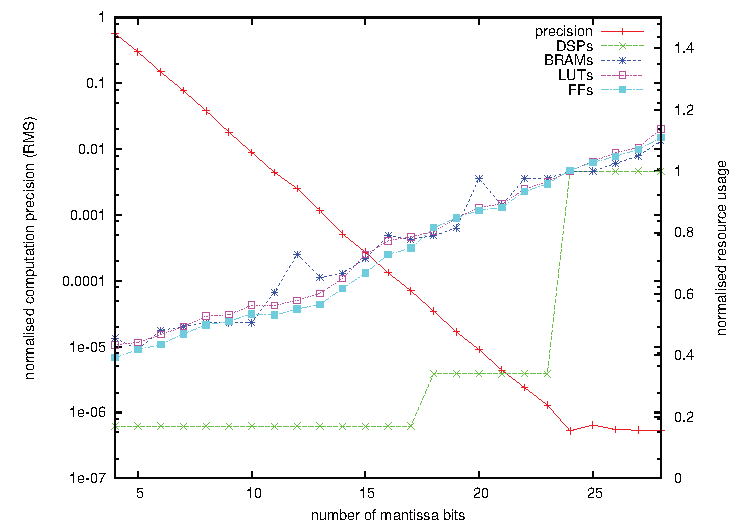
\includegraphics[scale=0.7]{figs/pre}
\caption{Exploration of accuracy vs resource usage trade-offs.}
\label{fig:precision}
\end{figure}

\begin{comment}
\begin{table}[!h]
  %  \renewcommand{\arraystretch}{1.1}
  \centering
  \caption{Results of varying the word length.}
  \label{table:aspect-wl}
  \begin{tabular}{ p{1cm} p{1cm} p{1cm} p{1cm} p{1cm}  p{1cm} }
    Word Width & LUT               & FF                & BRAM           & DSP             & Relative Error \\ \hline
    8, 24      & 106033  (35.63\%) & 143508  (24.11\%) & 295  (27.73\%) & 702  (34.82\%)  & \TODO          \\
    8, 22      & 133973  (45.02\%) & 185520  (31.17\%) & 295  (27.73\%) & 306  (15.18\%)  & \TODO          \\
    8, 20      & 129581  (43.54\%) & 178333  (29.96\%) & 289  (27.16\%) & 306  (15.18\%)  & \TODO          \\
    8, 18      & 121439  (40.81\%) & 170721  (28.68\%) & 286  (26.88\%) & 306  (15.18\%)  & \TODO          \\
    8, 16      & 117904  (39.62\%) & 157359  (26.44\%) & 283  (26.60\%) & 204  (10.12\%)  & \TODO          \\
  \end{tabular}
\end{table}
\end{comment}

Design space exploration using the parallelism aspect can be used to
illustrate design scalability. Figure \ref{fig:scalability} shows that
performance scales linearly with the number of parallel
pipelines. This type of exploration can also be used to expose
bottlenecks. This aspect can be combined with others such as adjusting
memory and stream frequency to understand the combined effect of these
optimizations. This would be useful in investigating the trade-off of
performance versus compilation time. In particular, it is not always
necessary to use maximum stream or memory frequency (e.g. in the case
of memory or compute bound applications respectively) but this can
significantly increase compilation time.

\begin{comment}
\begin{figure}[!h]
  \centering
  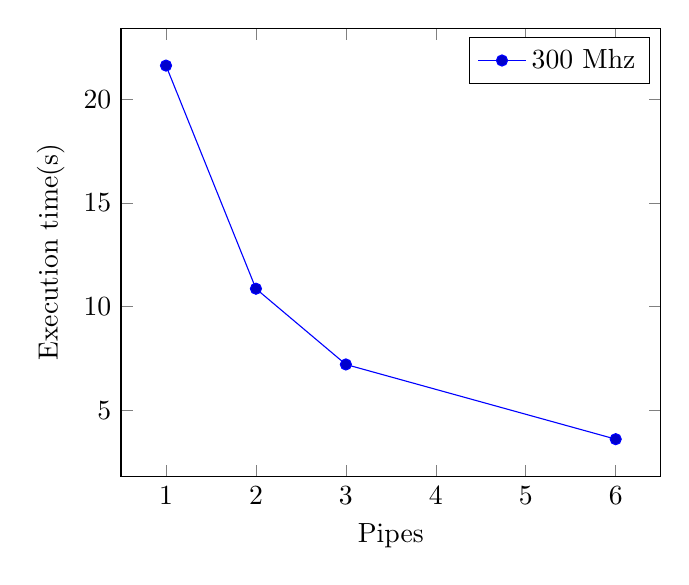
\begin{tikzpicture}
    \begin{axis}[xlabel=Pipes,ylabel=Execution time(s)]
      \addplot coordinates {
        (1, 21.630226)
        (2, 10.86542)
        (3, 7.210907)
        (6, 3.606188)
      };
      \legend{300 Mhz, 333 Mhz. 400 Mhz}
    \end{axis}
  \end{tikzpicture}
  \caption{Scalability of the MaxC dataflow design -- performance
    increases linearly with the number of parallel pipelines.}
  \label{fig:scalability}
\end{figure}
\end{comment}


The DSP aspect allows to explore the resource trade-offs of
implementing arithmetic operations in either DSPs or LUTs and FFs as
shown in Figure \ref{fig:arith}. This can help avoiding over mapping
on DSPs for arithmetic intensive applications.

\begin{figure}[!h]
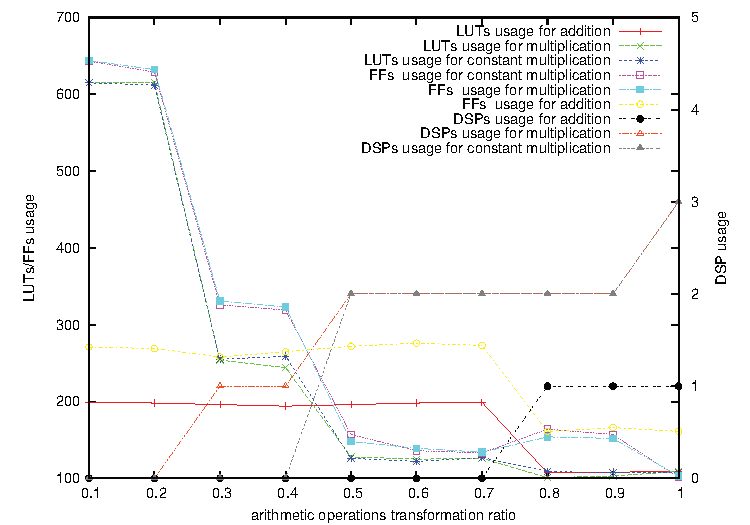
\includegraphics[scale=0.7]{figs/arith}
\caption{Exploration of DSP and LUT/FF balancing for arithmetic
  operations.}
\label{fig:arith}
\end{figure}

Finally table \ref{speedup} shows speedups obtained by the MaxC
dataflow design compared to CPU, GPU and other FPGA
implementations. This shows that our approach can match the
performance of the static reference version achieving a significant
speedup of up to 50x over software only versions.

\begin{table}[!h]
  \renewcommand{\arraystretch}{1.1}
  \centering
  \caption{Execution time, throughput and speed up results for RTM compared to CPU and GPU
    implementations (Sizes s = 128x128x128, m=128x256x256,
    l=256x512x512, 1000 iterations). Results are shown for both the static (S) and run-time reconfigurable version (R).}
  \label{speedup}
  \begin{tabular}{p{1cm}|cc|cc|cc|cc}
    \hline
    \multirow{2}{*}{\bf{Size, Pipes} }           &
    \multicolumn{2}{c|}{\bf{Time(s)}} & \multicolumn{2}{c|}{\bf{GFLOP/s}} &
    \multicolumn{2}{c|}{\bf{vs CPU}}  & \multicolumn{2}{c}{\bf{vs GPU}}                                                      \\
                                      &                               S      & R & S     & R & S     & R & S    & R    \\\hline \hline
    S, 12                                                              & 1.80   & - & 70.6  & - & 50.4  & - & 1.09 & 1.14 \\
    S, 6                                                                 & 3.60   & - & 35.3  & - & 25.2  & - & 0.54 & 0.57 \\
    S, 3                                                                 & 7.21   & - & 17.6  & - & 12.6  & - & 0.27 & 0.28 \\
    S, 2                                                                 & 10.86  & - & 11.73 & - & 8.4   & - & 0.18 & 0.18 \\
    S, 1                                                                 & 21.63  & - & 5.86  & - & 4.2   & - & 0.09 & 0.09 \\ \hline
    M, 12                                                               & 9.1    & - & 68.2  & - & 81    &   & 1.05 & 1.35 \\
    M, 6                                                                 & 18.21  & - & 34.1  & - & 40.5  &   & 0.52 & 0.67 \\
    M, 3                                                                 & 36.44  & - & 17.05 & - & 20.25 &   & 0.26 & 0.33 \\
    M, 2                                                                 & 72.91  & - & 11.36 & - & 13.5  &   & 0.17 & 0.22 \\
    M, 1                                                                 & 145.76 & - & 5.68  & - & 6.75  &   & 0.08 & 0.11 \\ \hline
    L, 12                                                               & 147.91 & - & 66.8  & - & 37.6  &   & 1.03 & 1.52 \\
    L, 6                                                                 & 295.6  & - & 33.4  & - & 18.8  &   & 0.51 & 0.76 \\
    L, 3                                                                 & 590.6  & - & 16.7  & - & 9.4   &   & 0.25 & 0.38 \\
    L, 2                                                                 & 1183.8 & - & 8.35  & - & 6.26  &   & 0.17 & 0.25 \\
    L, 1                                                                 & 2366.4 & - & 4.17  & - & 3.13  &   & 0.08 & 0.12 \\\hline \hline

  \end{tabular}
\end{table}
